\documentclass[12pt,a4paper]{article}
\usepackage[a4paper, portrait, margin=1in]{geometry}
\usepackage{hyperref}
\usepackage{fancyhdr}
\usepackage{graphicx}
\usepackage{pdflscape}
\usepackage{svg}
\usepackage{wrapfig}
\usepackage{lastpage}
\usepackage[autostyle]{csquotes}

\MakeOuterQuote{"}
\graphicspath{ {./} }
\hypersetup{
	colorlinks=true,
	linkcolor=blue,
	filecolor=magenta,
	urlcolor=blue,
	pdftitle={Projeto AMS 2022/2023 - Entrega 2 - Grupo 38},
	pdfpagemode=FullScreen,
}

\pagestyle{fancy}
\fancyhf{}
\fancyhead[C]{Projeto AMS 2022/2023 - Entrega 2 - Grupo 38}
\fancyfoot[C]{99209, 99256, 99311}
\fancyfoot[R]{Pág. \thepage{} de \pageref*{LastPage}}

\begin{document}

\begin{titlepage}
	\begin{center}

		\vspace*{0.5cm}
		
\includegraphics[width=0.5\textwidth]{ist-logo.png}

		\vspace{1cm}
		\Huge
		\textbf{Projeto de AMS: Entrega 2}

		\vspace{0.5cm}
		\LARGE
		Grupo 38 \quad | \quad Turno L08 \quad | \quad 2022/2023

		\vfill
	\end{center}

	\large
	\begin{tabular}{c|c|c}
		\textbf{Nome}           & \textbf{Número} & \textbf{Est. Horas Trabalho} \\
		\hline
		Diogo Romão Cardoso     & 99209           & 19h                          \\
		João Fernandes Rocha    & 99256           & 19h                          \\
		Rafael Serra e Oliveira & 99311           & 19h
	\end{tabular}

	\vspace{5cm}
\end{titlepage}

\begin{landscape}
	\section*{B.1.1. Diagrama de Vista Geral do Negócio}
	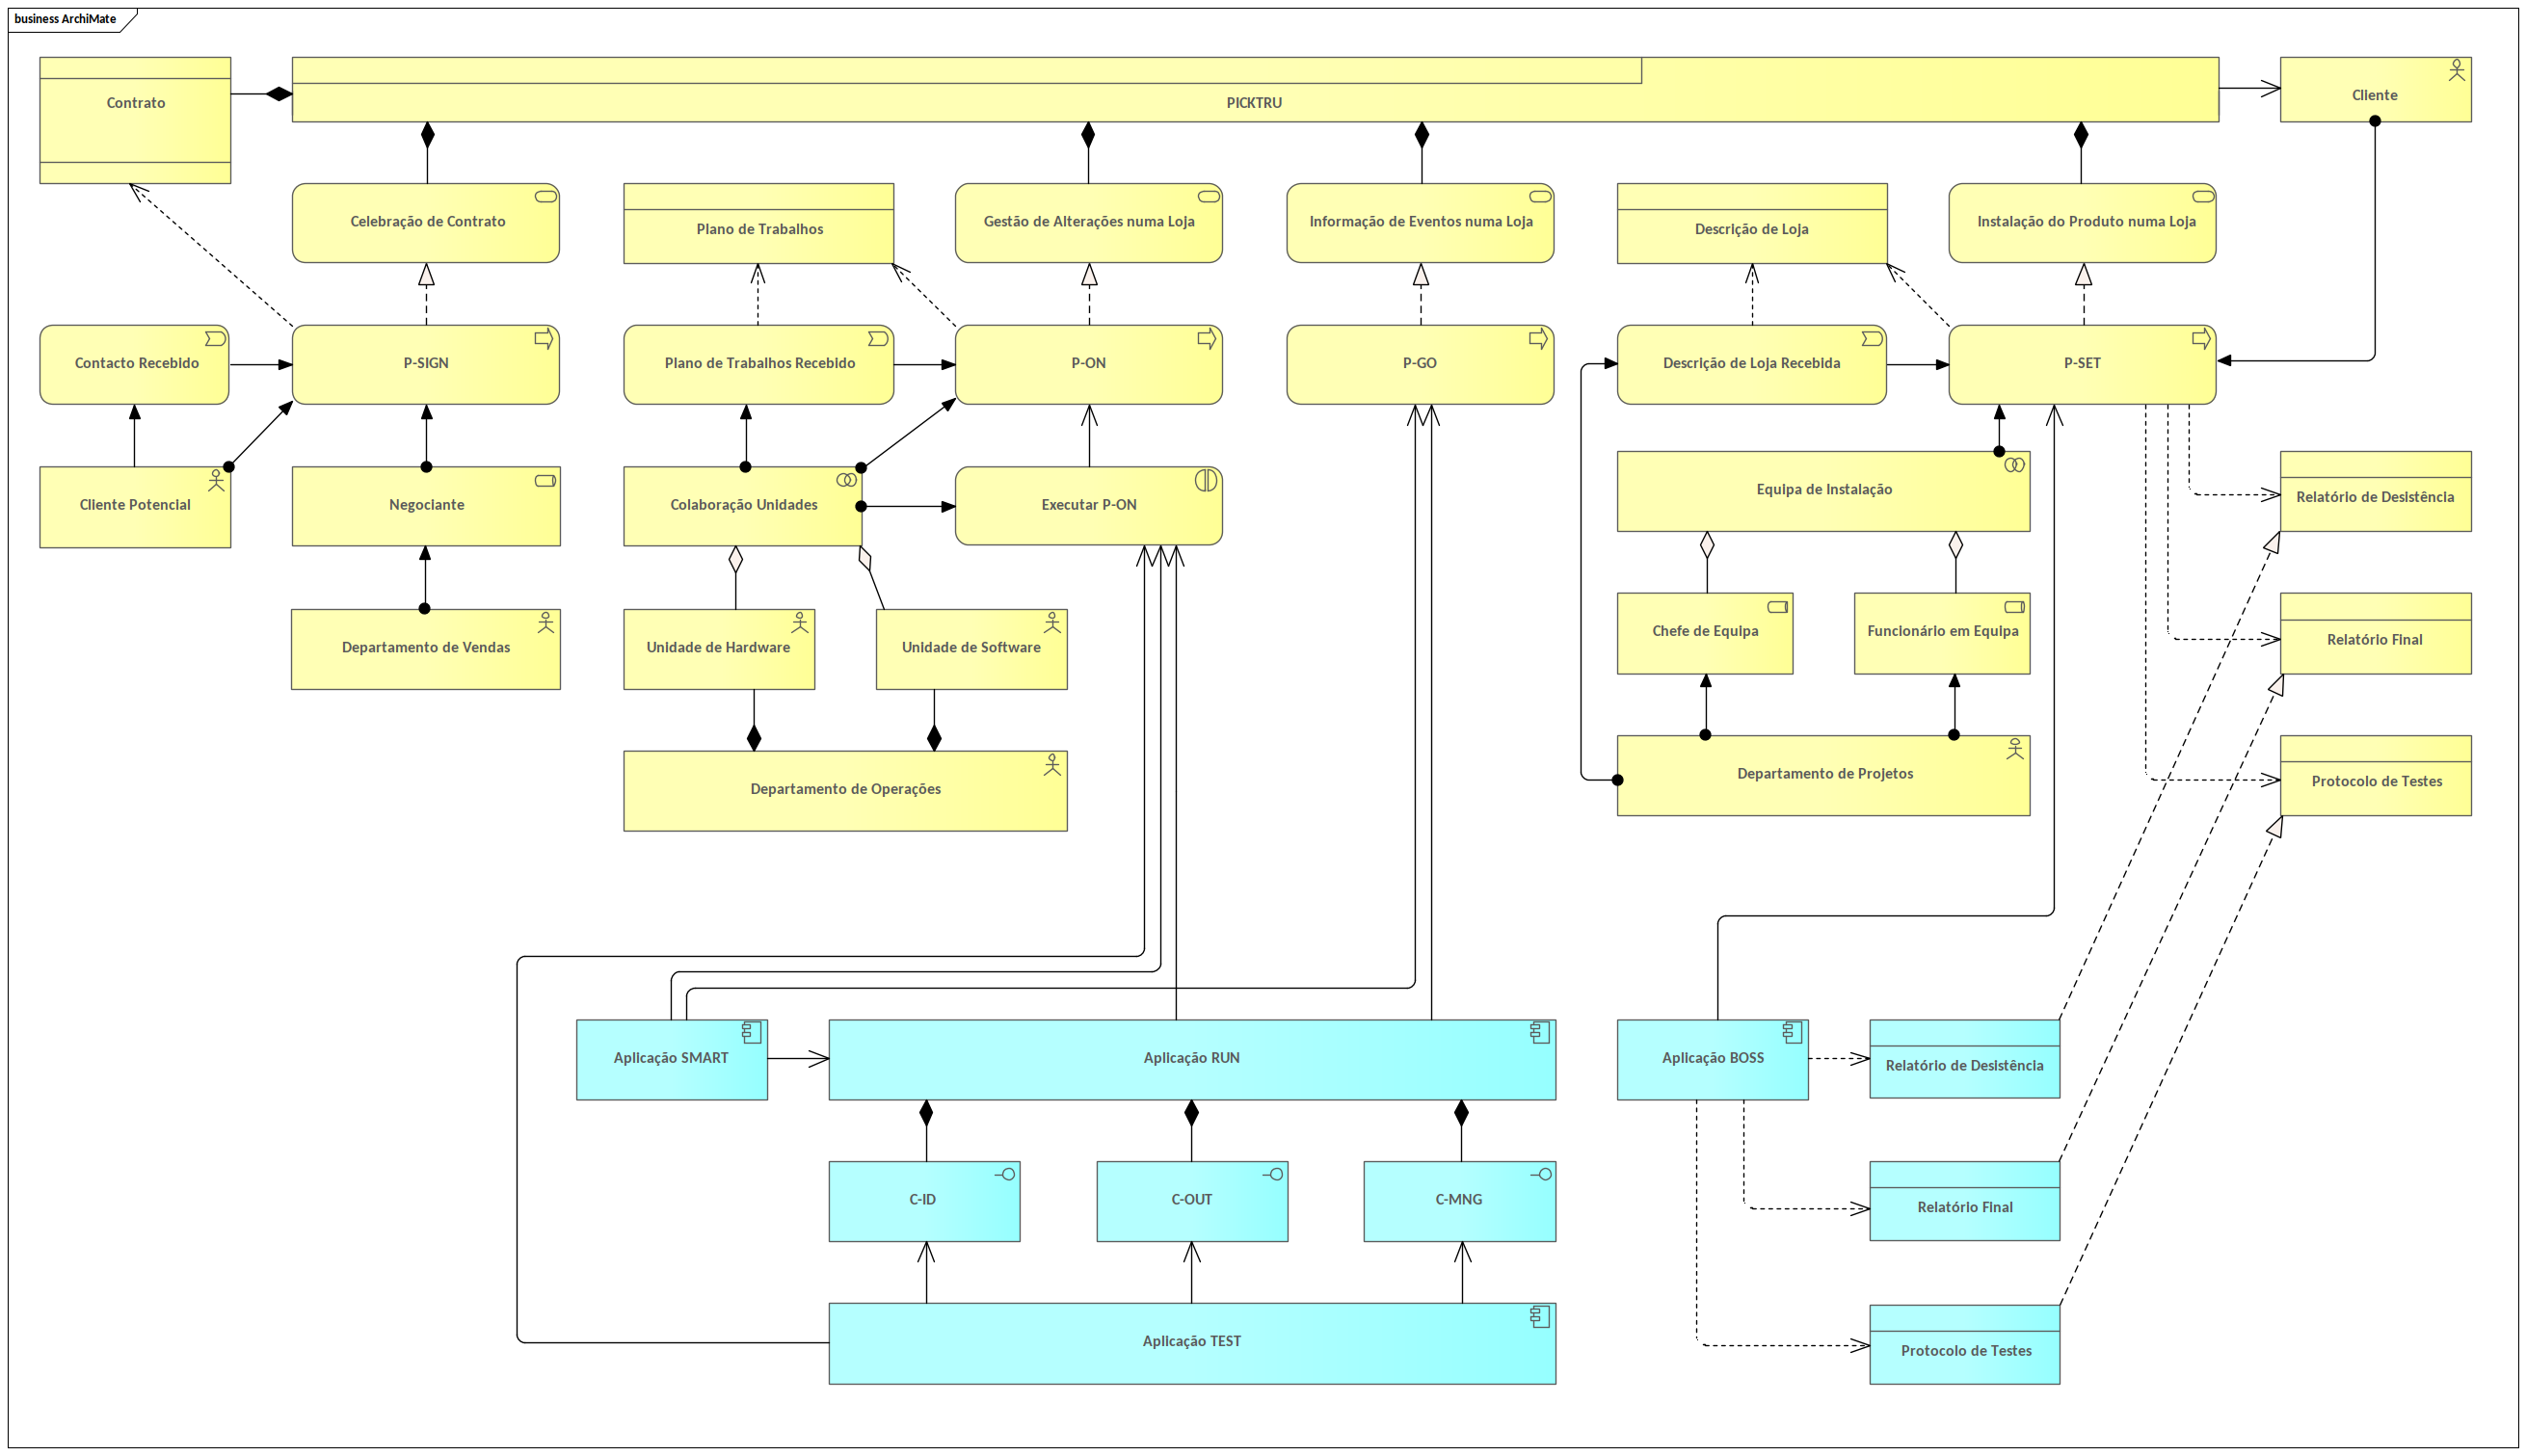
\includegraphics[width=1.59\textwidth]{../ArchiMate.png}
\end{landscape}

\begin{landscape}
	\section*{B.1.2. Diagrama do Processo P-SET}
	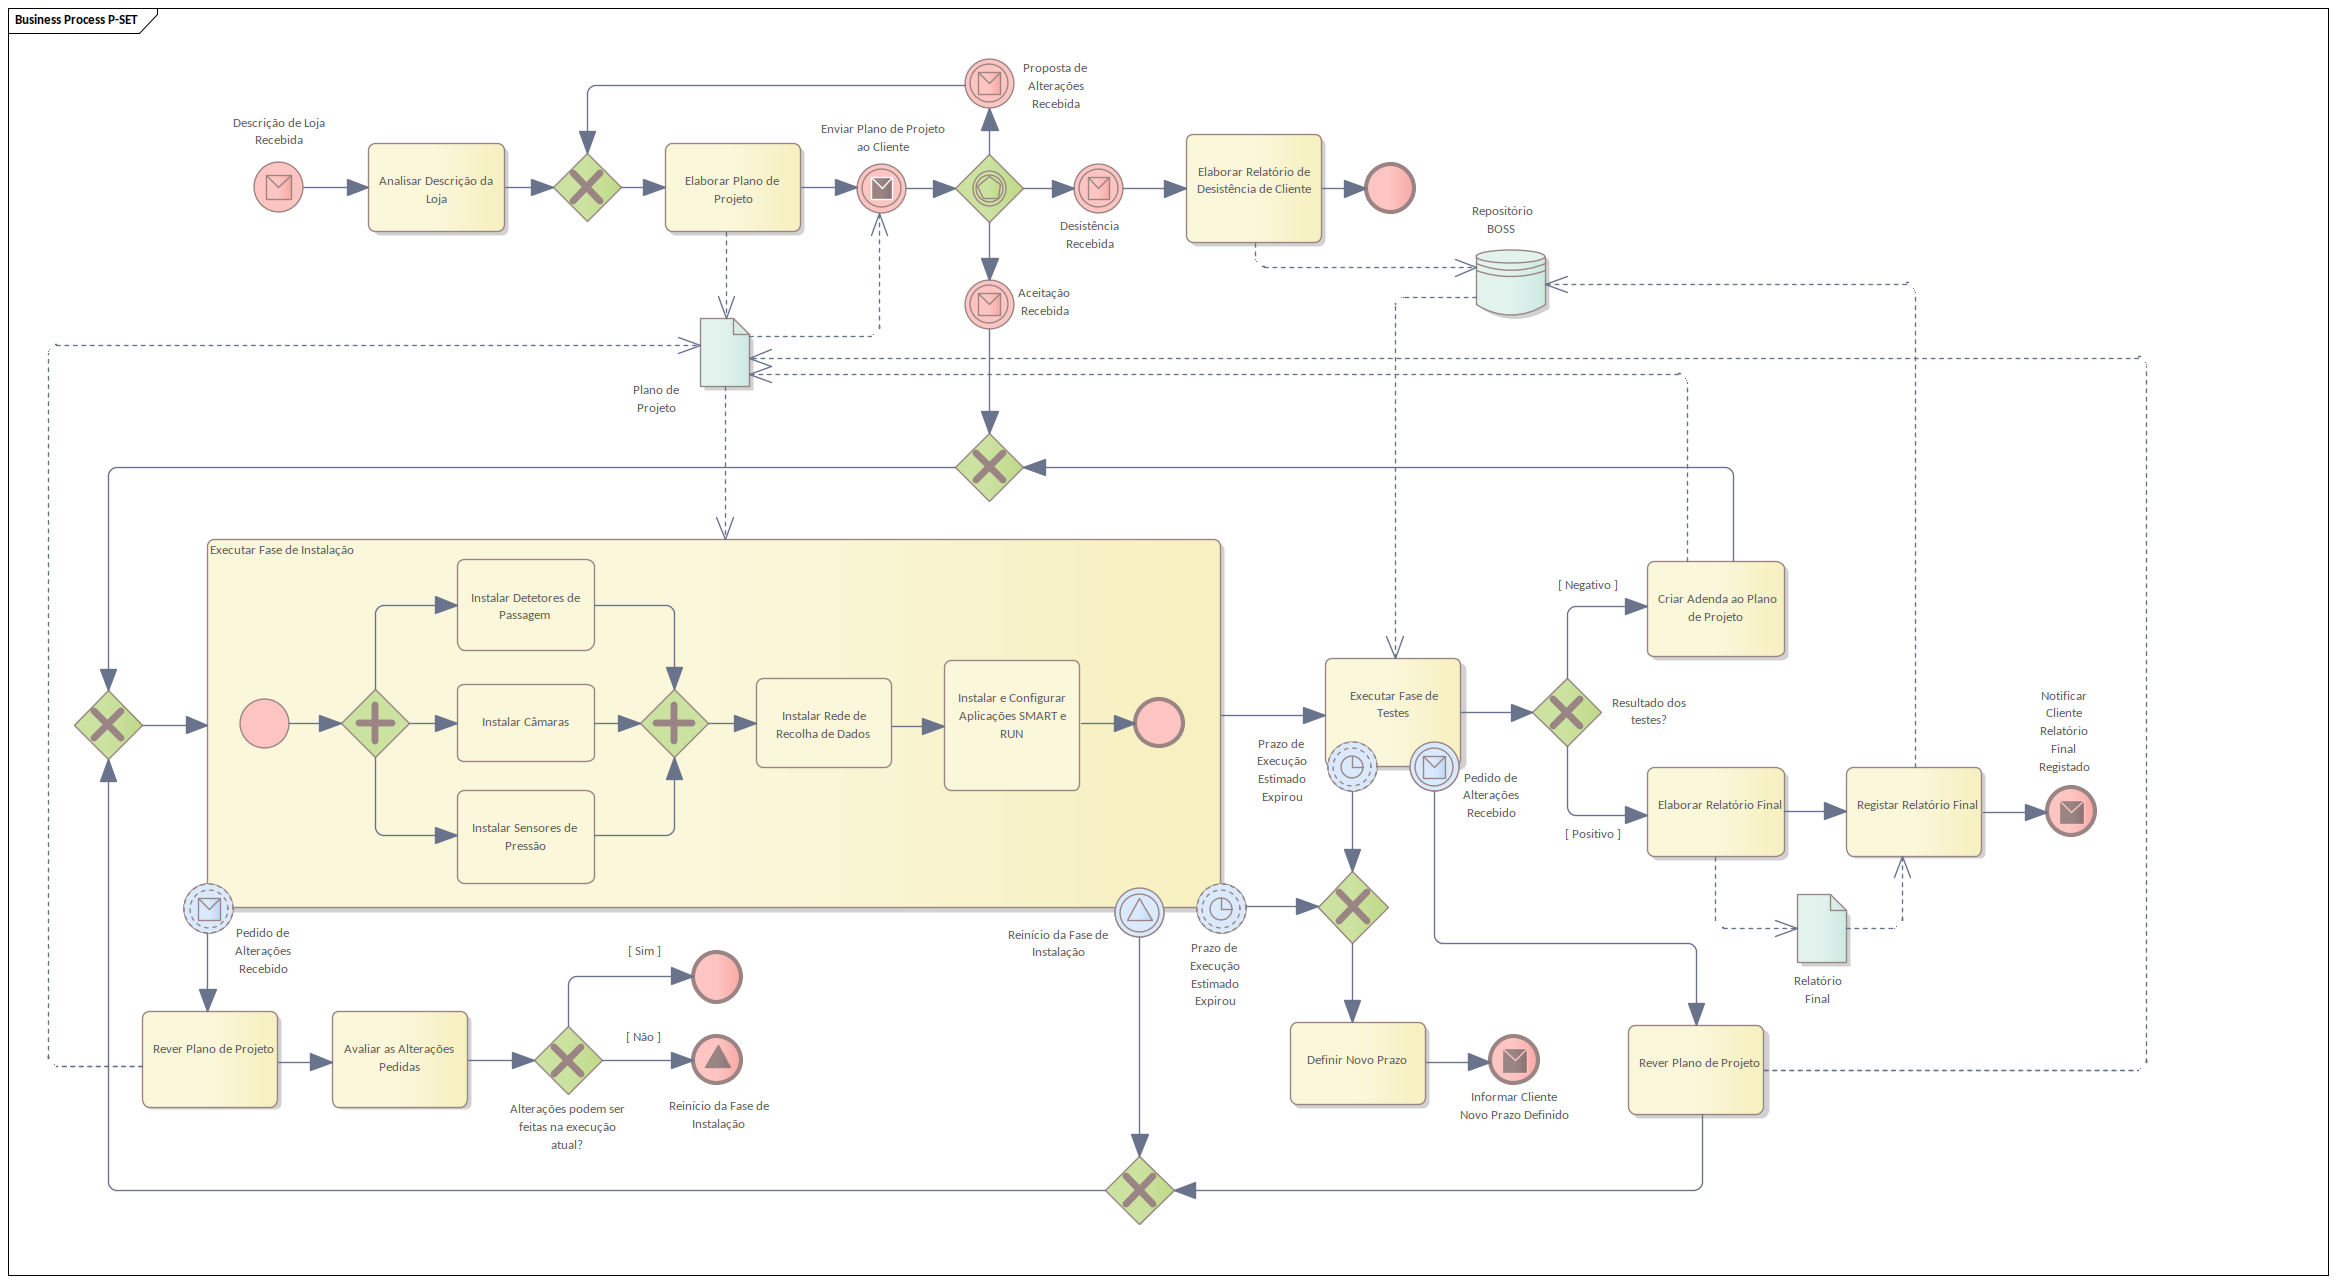
\includegraphics[width=1.59\textwidth]{../BPMN_P-SET.png}
\end{landscape}

\begin{landscape}
	\section*{B.1.2. Diagrama do Processo P-ON}
	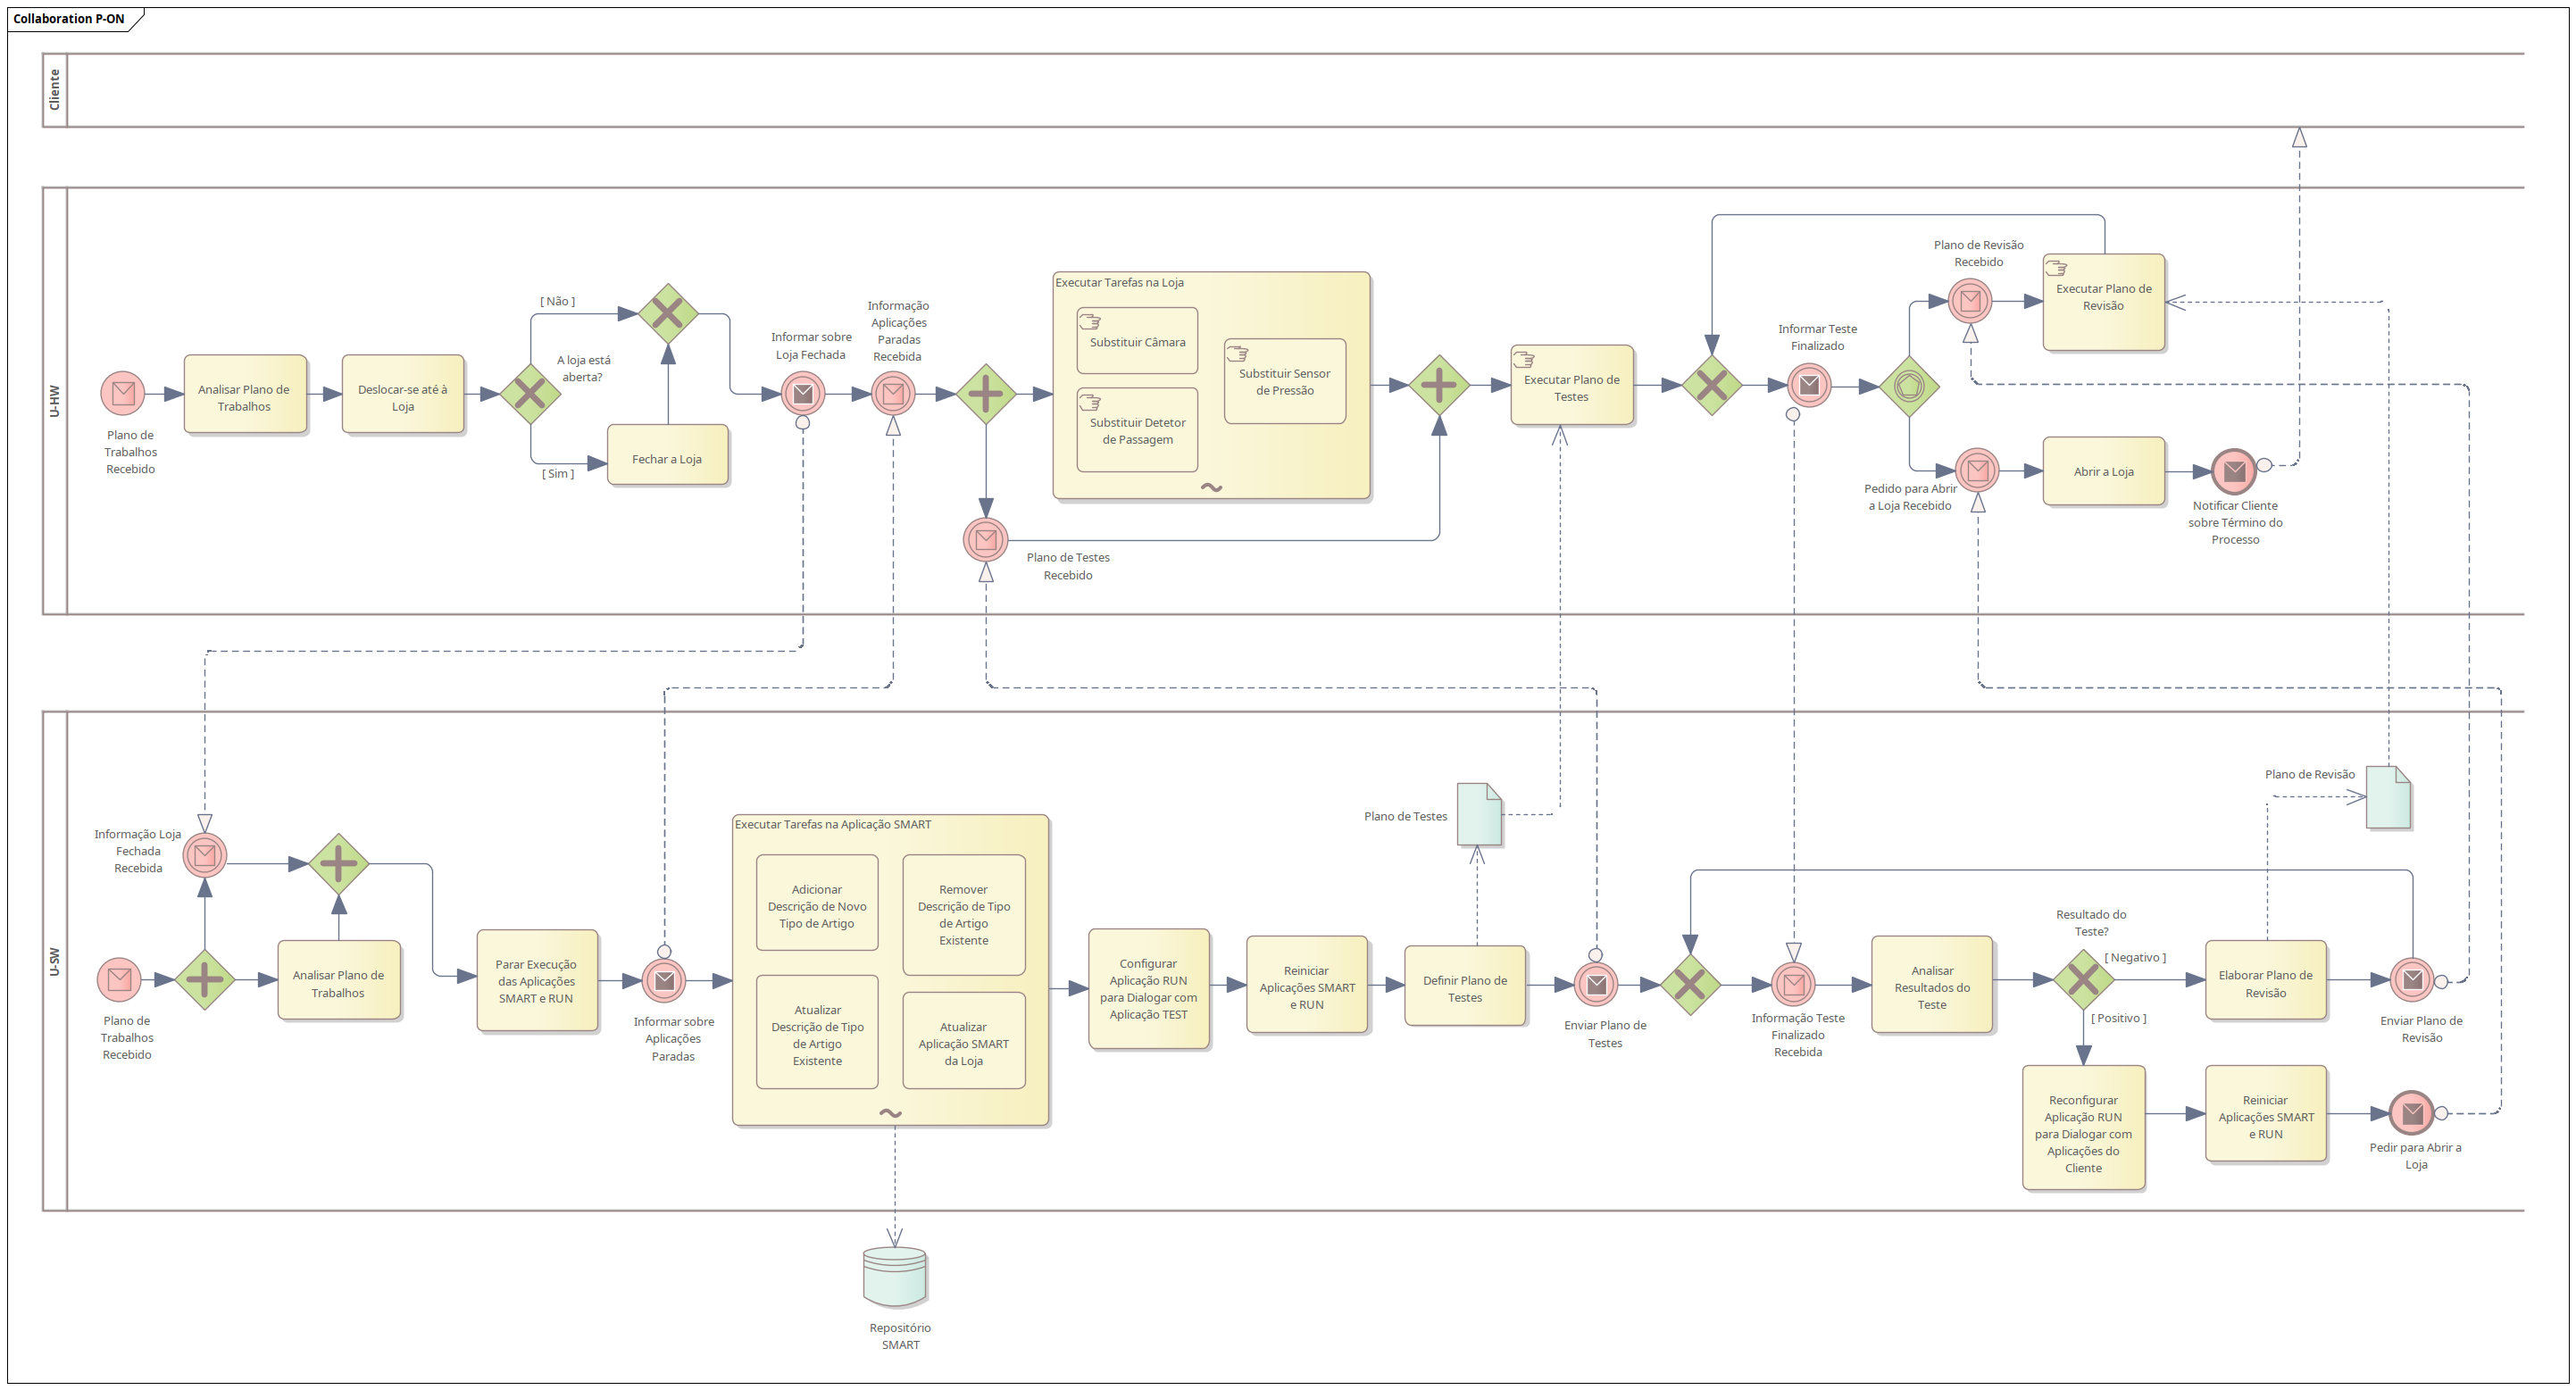
\includegraphics[width=1.59\textwidth]{../BPMN_P-ON.png}
\end{landscape}

\begin{landscape}
	\section*{B.2.1. Diagrama de Casos de Uso: Sistema RUN}
	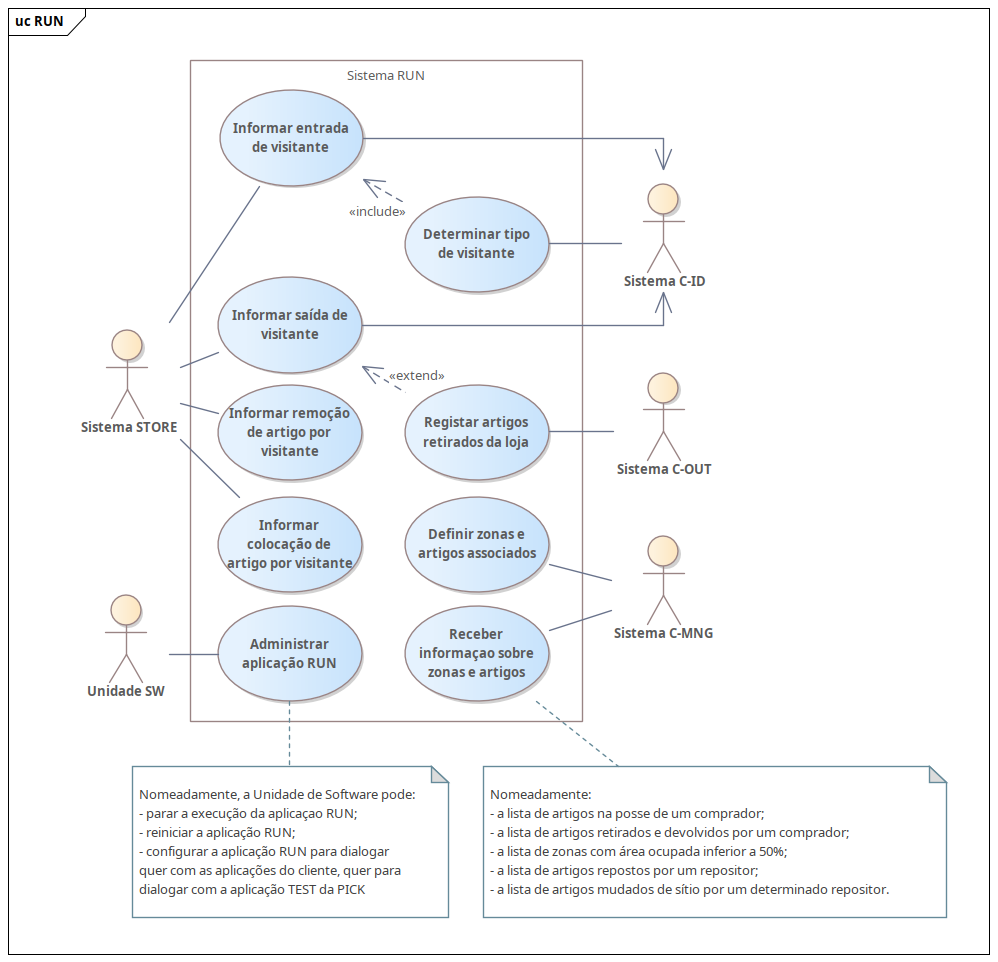
\includegraphics[width=1.59\textwidth]{../UC_RUN.png}
\end{landscape}

\begin{landscape}
	\section*{B.2.2. Diagrama de Casos de Uso: Sistema STORE}
	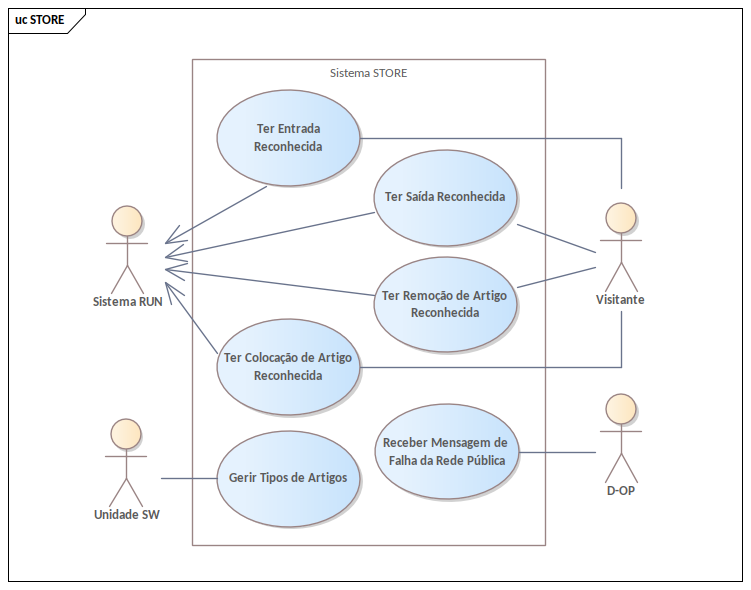
\includegraphics[width=1.19\textwidth]{../UC_STORE.png}
\end{landscape}

\begin{landscape}
	\section*{B.3. Diagrama de Classes: Aplicação RUN}
	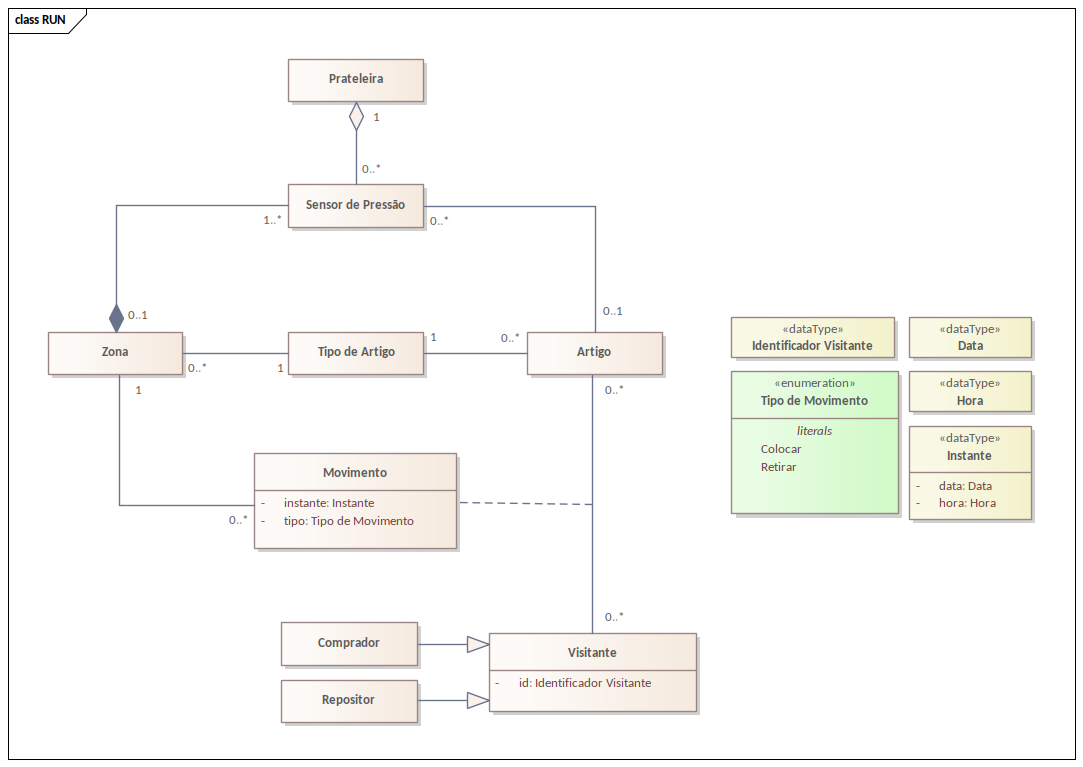
\includegraphics[width=1.26\textwidth]{../Class_RUN.png}
\end{landscape}

\begin{landscape}
	\section*{B.4. Diagrama de Máquina de Estados: Zona (Aplicação RUN)}
	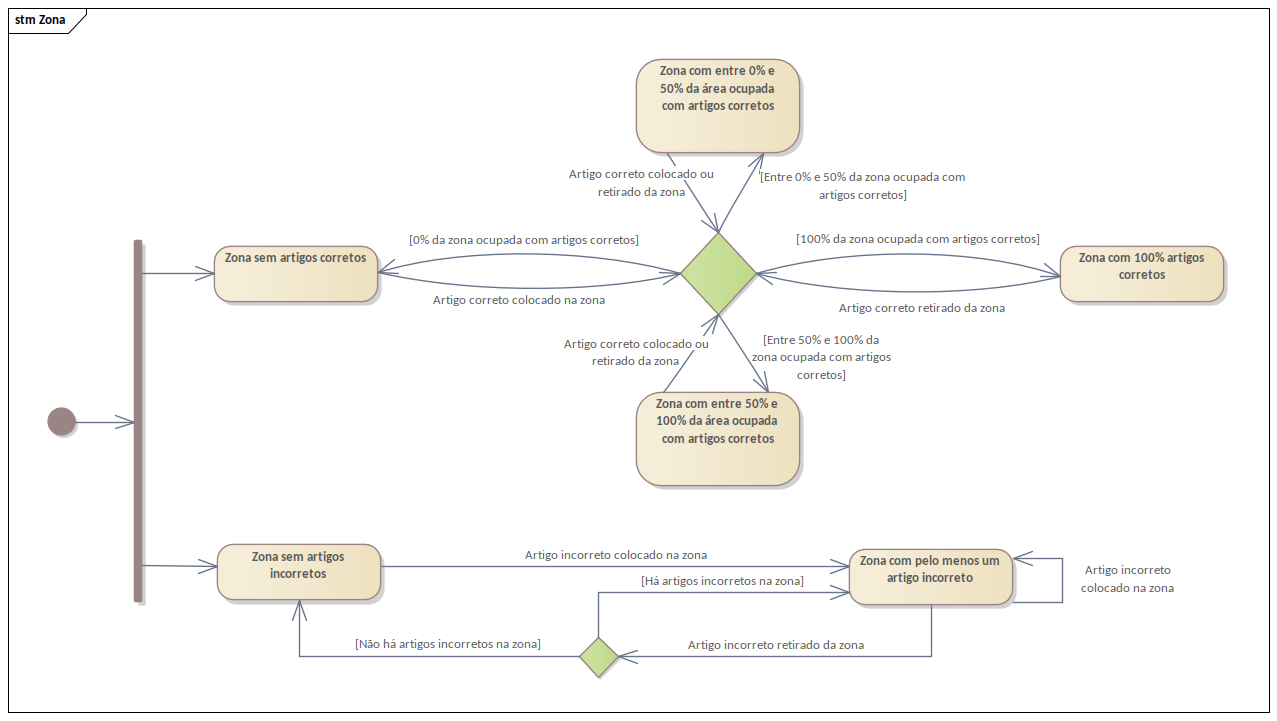
\includegraphics[width=1.59\textwidth]{../State_Zona.png}
\end{landscape}

\begin{landscape}
	\section*{B.5. Diagrama de Blocos: Sistema STORE}
	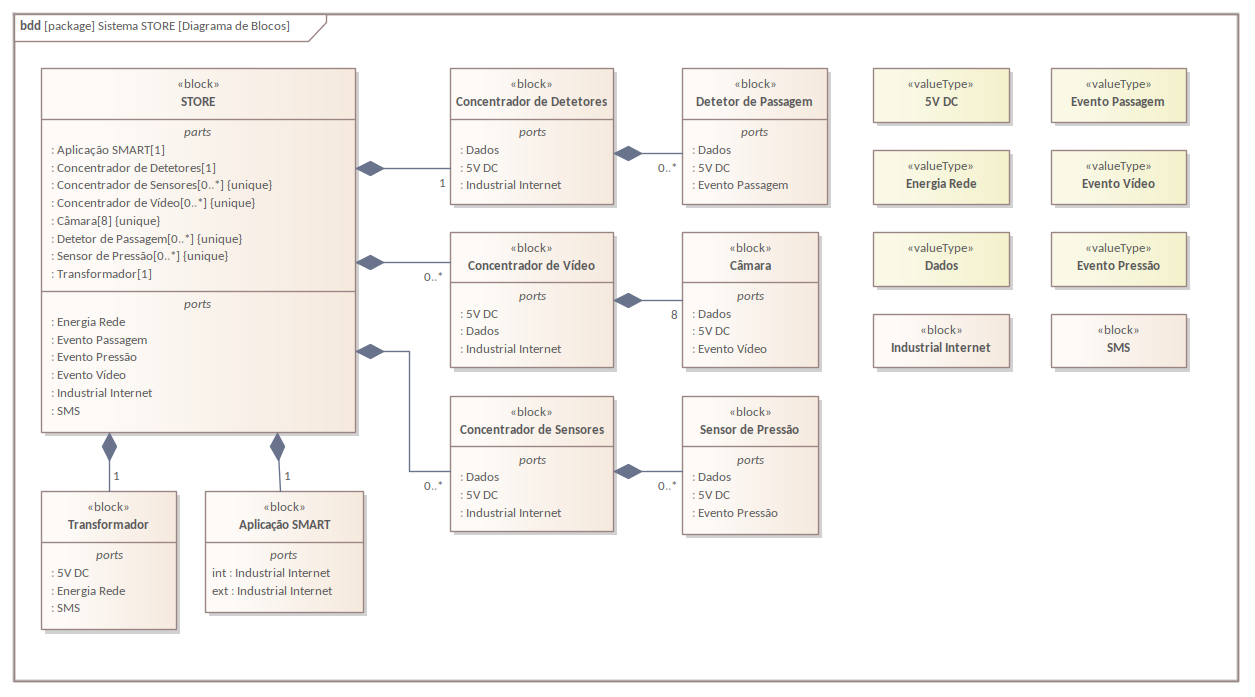
\includegraphics[width=1.45\textwidth]{../BDD_STORE.png}
\end{landscape}

\begin{landscape}
	\section*{B.6. Diagrama Interno de Blocos: Sistema STORE}
	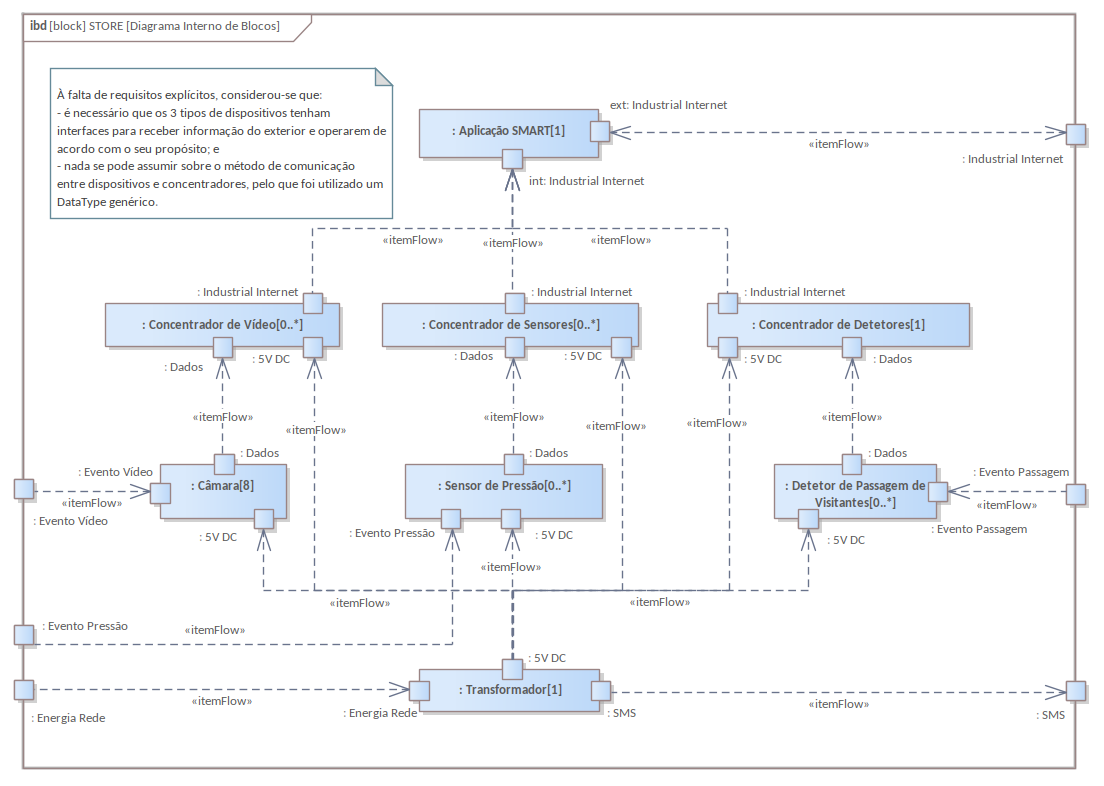
\includegraphics[width=1.25\textwidth]{../iBD_STORE.png}
\end{landscape}

\end{document}